\documentclass[border=10pt]{standalone}
\usepackage{tikz,times}
\usepackage{ctex}
\usepackage{pgfplots}
\pgfplotsset{compat=1.16}
\usepackage{xcolor}
\usepackage{filecontents}
\usepackage{amsmath}
\usetikzlibrary{snakes}
\usepgfplotslibrary{groupplots}
\begin{document}
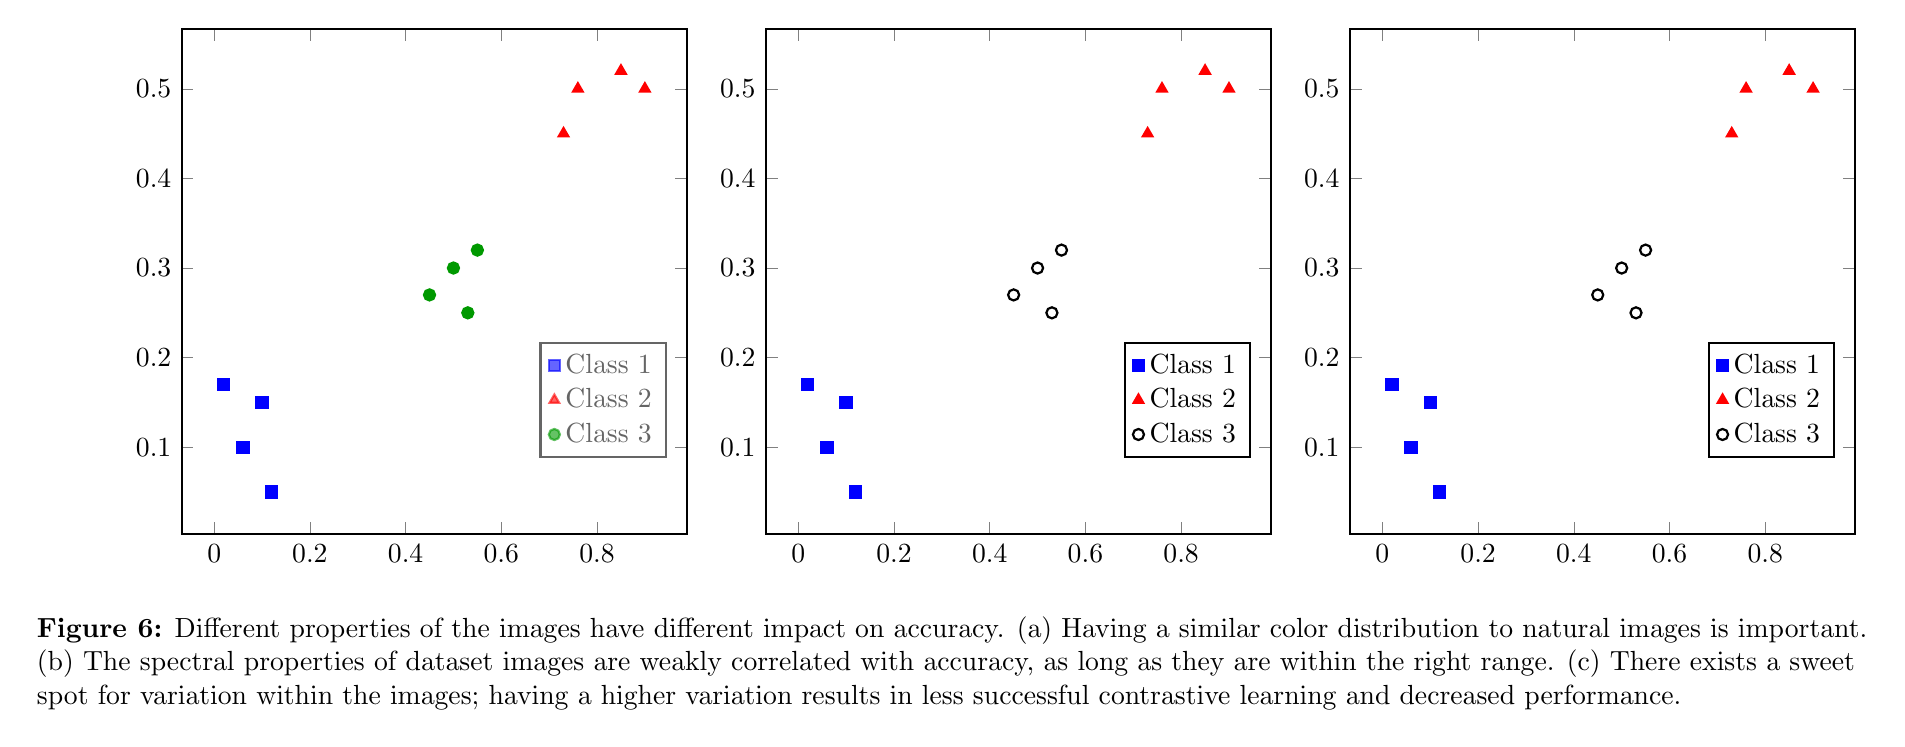
\begin{tikzpicture}
\pgfplotsset{
width=8cm,
height=8cm,
every axis legend/.append style={
    at={(0.96,0.15)},
    fill=white,
    font=\normalsize,
    opacity=0.6,
    anchor=south east},
     every axis title/.append style={
 at={(2.2,-0.4)},
    fill=white,
    font=\normalsize,
    opacity=1,
    anchor=south east,
    align=left
    },
    every axis y label/.append style={at={(0.04,0.5)}}
    }
\begin{groupplot}[group style={group size=3 by 1}]
%1
% #########################################
    \nextgroupplot[scatter/classes={
    a={mark=square*,blue},%
    b={mark=triangle*,red},%
    c={mark=*,green!60!black}},
    thick
    ]
    \addplot[scatter,only marks,
    scatter src=explicit symbolic]
    coordinates {
    (0.1,0.15)  [a]
    (0.45,0.27) [c]
    (0.02,0.17) [a]
    (0.06,0.1)  [a]
    (0.9,0.5)   [b]
    (0.5,0.3)   [c]
    (0.85,0.52) [b]
    (0.12,0.05) [a]
    (0.73,0.45) [b]
    (0.53,0.25) [c]
    (0.76,0.5)  [b]
    (0.55,0.32) [c]
    };
    \legend{Class 1,Class 2,Class 3,Line}

%2
% #########################################
    \nextgroupplot[scatter/classes={
    a={mark=square*,blue},%
    b={mark=triangle*,red},%
    c={mark=o,draw=black}},
    every axis legend/.append style={
    at={(0.96,0.15)},
    fill=white,
    font=\normalsize,
    opacity=1,
    anchor=south east},
     title={{\bf Figure 6:} Different properties of the images have different impact on accuracy. (a) Having a similar color distribution to natural images is important.\\ (b) The spectral properties of dataset images are weakly correlated with accuracy, as long as they are within the right range. (c) There exists a sweet\\ spot for variation within the images; having a higher variation results in less successful contrastive learning and decreased performance.},
    thick
    ]
    % \addplot[] is better than \addplot+[] here:
    % it avoids scalings of the cycle list
    \addplot[scatter,only marks,
    scatter src=explicit symbolic]
    coordinates {
    (0.1,0.15)  [a]
    (0.45,0.27) [c]
    (0.02,0.17) [a]
    (0.06,0.1)  [a]
    (0.9,0.5)   [b]
    (0.5,0.3)   [c]
    (0.85,0.52) [b]
    (0.12,0.05) [a]
    (0.73,0.45) [b]
    (0.53,0.25) [c]
    (0.76,0.5)  [b]
    (0.55,0.32) [c]
    };
    \legend{Class 1,Class 2,Class 3,Line}

%3
% #########################################
    \nextgroupplot[scatter/classes={
    a={mark=square*,blue},%
    b={mark=triangle*,red},%
    c={mark=o,draw=black}},
    every axis legend/.append style={
    at={(0.96,0.15)},
    fill=white,
    font=\normalsize,
    opacity=1,
    anchor=south east},
    thick
    ]
    % \addplot[] is better than \addplot+[] here:
    % it avoids scalings of the cycle list
    \addplot[scatter,only marks,
    scatter src=explicit symbolic]
    coordinates {
    (0.1,0.15)  [a]
    (0.45,0.27) [c]
    (0.02,0.17) [a]
    (0.06,0.1)  [a]
    (0.9,0.5)   [b]
    (0.5,0.3)   [c]
    (0.85,0.52) [b]
    (0.12,0.05) [a]
    (0.73,0.45) [b]
    (0.53,0.25) [c]
    (0.76,0.5)  [b]
    (0.55,0.32) [c]
    };
    \legend{Class 1,Class 2,Class 3,Line}

 \end{groupplot}
    \end{tikzpicture}
\end{document} 